%préambule
%chargement des packages
\documentclass[a4paper, 12pt, hidelinks]{article}

%Langage et typo
\usepackage[babel]{microtype}
\usepackage[english]{babel}

%Gestion grahique
\usepackage{graphicx}
\usepackage{mathspec}
\graphicspath{{./Figures/}}


%Gestion des tables
\usepackage{array}
\usepackage{rotating}
\usepackage{afterpage}
\usepackage{multirow}
\usepackage{adjustbox}

 %Pour les qques formules
\usepackage{mathspec}

%Définition des paramètres de mise en page
%Interlignes
\usepackage{setspace}
\onehalfspace

%Marges
\usepackage[margin=2.5cm]{geometry}

%%Font
%\usepackage{fontspec}
\setmainfont{Times New Roman}
%Couleurs
\usepackage[svgnames]{xcolor}

%Gestion des titres de partie et des numérotations
\usepackage{titlesec}% http://ctan.org/pkg/titlesec
\titleformat{\section}%
  [hang]% <shape>
  {\normalfont\bfseries\Large}% <format>
  {}% <label>
  {0pt}% <sep>
  {}% <before code>
\renewcommand{\thesection}{}% Remove section references...
\renewcommand{\thesubsection}{\arabic{subsection}}

%Gestion biblio
\usepackage{natbib}
\usepackage[colorlinks = false, pagebackref = true]{hyperref}
\usepackage{url}
\setcitestyle{citesep={;},aysep={}}
\usepackage{multicol}

%Gestion annexe
\usepackage[toc,page]{appendix}


%Page de garde
\title{Rapport stage M2}
\author{Moi même}
\date{Mardi 9 février 2020}


\begin{document}
\maketitle
\newpage
\tableofcontents
\newpage


\section{Acknowledgements}
\section{Présentation de la structure d'accueil}
\newpage
\section{Literature review}
%!TEX root = ./Structure_rapport_final.tex


\subsection{Structure and dynamics of ecosystems: how can species coexist in same environment?} 

Of all the questions raised when it comes to study Nature, the most common yet complex one is “how do organisms and environment interact with each other?” \citep{sutherland2013}. In other words, what are the processes and rules that define structure and functioning of ecosystems? Taken as a whole, an ecosystem can be seen as a giant network: all individuals from every species are linked to one another through intra- and inter-specific relationships, that implies competition, parasitism, predation\ldots{}; and each individual is linked to its physical environment, on which it depends for food prospection, shelter and/or favorable conditions for breeding. The main purpose of ecology is to study those links and ultimately, to be able to map the central relationships and flows that are keys to maintain stable ecosystems \citep{albouy2011}. Community ecologists, regardless of the ecosystem they are studying, try to answer some fairly similar questions such as “how do species share environmental resources?” or “how can species relying on the same resource to thrive and survive can coexist?”. Indeed, the mere observation that species can live and develop a population without encroaching each other suggests that, even if species compete to access the same resources, the use of resources is balanced and allows stable relationships between species to develop. Most of all, if species depend on the same resources to survive, how can diversity within an ecosystem last over time?

\subsection{Concepts and definition for studying ecosystems’ dynamic.}
 
To answer those questions, the structure and dynamic of ecosystems need to be investigated and ecological concepts must be defined. \\ 
First, a ``community'' is made up of all living organisms (all species combined), which interact and occupy a specific habitat. Within this habitat, the concept of ``ecological niche'' reflects the fact that distinct populations use differently space and trophic resources to meet their needs. In 1917, Grinnell was the first to scientifically as ``ecological niche'' all the requirements that a species needs to thrive \citep{grinnell1917}.
This concept covers both biotic (food abundance and availability, competition within and among species, predation-prey relationships \ldots{}) and abiotic conditions (environmental factors such as temperature or pression, shelter availability \ldots{}), and it shapes the areas suited for species according to their needs. This definition is refined by \citet{hutchinson1957}: resources and their availability are the main drivers for the coexistence of species, since resources are essential for species to thrive and are therefore considered limiting factors. Furthermore, Hutchinson’s definition distinguishes the concepts of (i)``fundamental niche'', which is a potential niche for a given species that offers all the optimal conditions for that species to flourish and (ii) ``realized niche'', which corresponds to the actual resources used by a species and which is often smaller than the fundamental niche, mainly because of competition between species. If resources are limited, competition between species that seek to simultaneously exploit the same resources may arise, either because they hunt the same prey or because they live in the same specific habitat and are therefore more likely to meet \citep{blondel1979}. When the resources are abundant enough, species may be able to share it without entering competition \citep{nagelkerke2018}. According to competition theory, community structures are defined by the way species are able to share or not resources. Therefore, to study the structure and dynamics of community and to identify the main factors that enable species to coexist, it is essential to determine the degree by which species share resources, in other words, quantify the overlap between ecological niches \citep{geange2011}. 


\subsection{Tools to study diversity in ecosystems and their limits}

Niche overlap can be approached from the habitat (beta overlap) or food (alpha overlap) perspective \citep{mouillot2005}. In both cases, a high degree of overlap means that the species are likely to compete for the same resources making their coexistence virtually impossible. Conversely, a low deree of overlap tends to suggest that species, even if they rely in part on the same resources, have a sufficiently wide range of accessible resources not to compete with each other \citep{mouillot2005}. No overlap means that species occupy distinct niches, are likely to use very different resources and that no competition is expected (see \ref{fig:lr1}. This approach has been widely developed over the last decades to study the distribution of abundance and the mechanisms favoring species coexistence, in particular to predict the impact of disturbances, such as the introduction of invasive species or climate change \citep{albouy2011,geange2011, martini2020}. 
\begin{figure} [!htbp]
	\begin{center}
		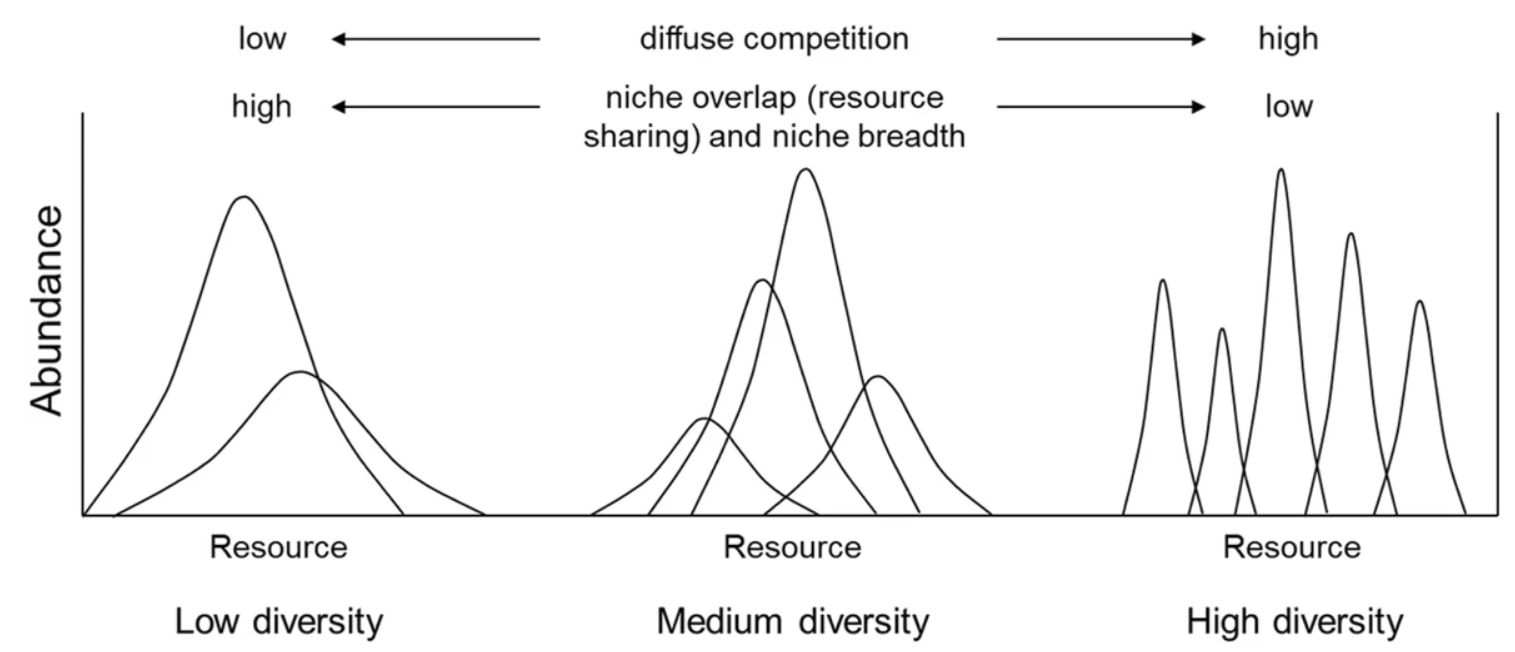
\includegraphics[width=0.8\textwidth]{niche_overlap.png}
	\end{center}
	\caption[Caracteristics of niches along a resource gradient]{Caracteristics of niches along a resource gradient at different levels of species diversity, from \citet{kim2020}.}
	\label{fig:lr1}
\end{figure}

To quantify niche overlap, several indices have been developed since the 60’s. Indices and threshold values are commonly used for studying specific, taxonomic or phylogenetic diversity. However, used alone, a result of diversity estimation through any index is usually poor and inaccurate, because complex and rich systems can not be described only by the result of a computation \citep{mejri2009}. Indeed, four of the best-known niche overlap indices, which are based on the intensity of utilisation of a resource use by species, were compared by \citet{linton1981} to assess the precision and accuracy: \citet{morisita1959} updated by \citet{horn1966}, \citet{schoener1968} and \citet{pianka1973}. Even if they lead to the same general conclusions, these four indices often give different results, because they use different computation parameters \citep{blondel1979}. Moreover, they are often highly sensitive to sample size, which adds uncertainty when it comes to interpreting their values \citep{linton1981}. Finally, \citet{grossman2009} points out that threshold values for those indices can be considered as arbitrary and might differ from one ecosystem to another, leading to an impossibility of comparing them. For all these reasons, using those indices to estimate if species share or not the same resources, and if so, how much is shared, does not seem relevant \citep{mouillot2005}. As such, they provide a qualitative assessment of the overlap rather than a quantitative one \citep{linton1981}.

Therefore, to understand how the structure and the dynamics of an ecosystem are defined and how such complex relationships can last for several generations, numerical models are often used (see Ecopath models, \url{https://ecopath.org}). This approach requires a simplification of the ecosystem, because simulating very complex models make the outcome virtually impossible to compute \citep{albouy2011}. Simplifying an ecosystem can be done in many ways: focusing on specific compartments of the ecosystem (\textit{e.g}: pelagic or benthic fauna), grouping species based on their trophic level, or taxonomy or similaire behavior \ldots{} Obviously, simplifying with any of these methods comes down to approximating the relationships and much of the complexity of an ecosystem, but if done properly, models are still able to produce reliable simulations of what is going on in real life \citep{albouy2011,evans2012,piroddi2015}. Yet, the main difficulty is to determine the criteria that are relevant to gather species and to simplify models. Whether they are too restrictive, or not enough, these criteria condition not only the accuracy of the model, but also its ability to be generalized \citep{moon2017,pease2015,pont2006}. For instance, if a model uses a taxonomic grouping of species, it will only be suited to study other ecosystems that contain the ame set of species or taxonomic groups. Its transposition to other unrelated ecosystems will thus be limited, if not impossible \citep{moon2017}. In the end, this modeling approach imposes a specific model for each ecosystem, which is highly time consuming and limits the possibilities of comparisons between ecosystems \citep{martini2020, mcgill2006}. Therefore, this approach remains very specific to a studied ecosystem and the species that compose it. 

%How does the morphology of fish impact its behaviour? 
%How can the morphology of the fish help us to understand more about its behaviour?

\subsection{Emergence of a more global approach based on functional traits.}

\subsubsection{General overview}

Community ecology aim to establish general rules explaining the functioning of communities. Species-centred approaches only provide information for a few specific systems but not general principles, that can be applied to a wide variety of communities or ecosystems \citep{albouy2011,martini2020}. Therefore, ecologists had to find a way to study ecosystems, to (i) give clues of how species interacts with each other and (ii) to assess how strongly species are related to their environment. Indeed, some scientists emphasized the urge to get rid of methods that were highly dependent of species, time or space, such as the ones described previously, and to use a more predictable and quantitative science that could play a major role in assessing global changes issues \citep{brindamour2011,mcgill2006,olden2002}. To this extend, \citet{mcgill2006} define a \textbf{trait} as a “well-defined, measurable property of organisms, usually measured at the individual level and used comparatively across species” and suggest that community ecology should try to understand how these traits interact with fundamental niches to define realized niches. The notion of ``trait'' has been widely used in the literature, but with slightly different meanings. For instance, \citet{violle2007} defined a trait as “any morphological, physiological or phenological feature measurable at the individual level, from cell to whole organism”. To ensure a consistent approach to community ecology studies, \citet{martini2020} suggests that the definition of \citet{violle2007} is precise enough, that it should serve as a reference and therefore should be used systematically. Yet, not all measurable traits provide the same information: for ecologists, traits that inform about (i) the interactions between species and the environment and (ii) the fitness of individuals are the most valuables \citep{kremer2017}. These specific traits are defined as “functional traits” and can relate to behavior, life history, morphology or physiology, influencing the general performances of organisms \citet{martini2020, mcgill2006}. They provide information on the main functions of organisms, such as acquisition of food or locomotion \citep{mejri2009}.

\subsubsection{Improvement of the method over the years}
The functional-traits approach was first developed in studies based on terrestrial plants. They showed that the morphology of species was correlated with their environment and that changes in their habitat could lead to changes of their morphology because this approach relies on the plasticity of traits \citep{boissezon2014,lavorel1997,martini2020}. Applied to aquatic animals, structure-function relationship has been well documented since the 1970s \citep{gosline1971, lagler1977, webb1984} and approaches based on morphological traits  seemed suitable to compare species \citep{norton1995} or to explore niches and compare communities \citep{winemiller1991}. For instance, \citet{albouy2011} developped a model to determine the diet of any marine species based on morphological traits, and thus establish trophic guilds. 
% Yet, the model could not predict diet overlap nor resource partitionning among species, because of intrinsic variability in the diet of fish. 

While the flexibility and intrinsic variabiliy of species should not be ignored, they can be hard to predict \citep{diderich2006,martini2020}. It is therefore essential to identify and select relevant traits, that can be used to explain most interactions between species and their environment. This is one of the main challenges of the functional traits approach, because the selected traits must be sufficiently variable beteen the levels being compared (species, populations, individuals …), and the observed variations must explain the actual differences in fitness or coexistence of species \citep{kremer2017}. \\

Yet, the flexibility in traits is what makes this approach so useful, as it allows for the quantification of intraspecific variability (especially when the environmental conditions change \citet{martini2020}) and interspecific variability that explains the interactions between species and their environment. In a nutshell, the traits to be used for functional trait approach must offer the best compromise between being (i) sufficiently informative with respect to the objectives, (ii) generic enough to be comparable across species --- even if they are very different morphologically --- and (iii) easily measurable to ensure repeatability between studies \citep{dumay2004, kremer2017}.

\subsection{The advent of functional diversity}
The functional approach is relatively recent. It developed in the 1980s with the collapse of populations, species extinctions and the biodiversity crisis \citep{wilson1988}. The functions performed by species began to be studied in greater depth when ecologists noticed that if a species disappeared from an ecosystem, it did not necessarily mean that the whole ecosystem was disturbed or even collapsed \citep{mejri2009}. The question ``Are all species essential for the proper functioning of ecosystems?'' became central, as did the need to define the role of species within ecosystems. In other words, can we consider that species are ``redundant" if they play the same role, fulfill the same function, in an ecosystem? To answer these questions, the functional trait approach seems relevant because it provides information on the roles of species in their environment, which is complementary to those provided by classical diversity indices, such as specific diversity, richness distribution or evenness \citep{marcon2015,mejri2009}. 

More importantly, functional traits and species role attribution are crucial in determining functional diversity, which is the primary factor explaining stability and productivity, and should therefore be preferred to specific or taxonomic diversity when studying community ecology \citep{dumay2004,mejri2009}. In fact, the resilience and health of ecosystems depends much more on the range of functions and functional traits exhibited by species than on the number of species \textit{per se} (i.e. species richness). Indeed, indices of specific abundance and diversity assume that all species are equivalent, and do not take into account the functions provided by these species \citep{mejri2009}. From this functional perspective, the richness of an ecosytem is determined by the extent of functional diversity provided by the species \citep{rocklin2004}. 

To estimate functional diversity, species must first be classified into ``functional groups'', which reflects the similarities of species according to 3 criteria. Within a functional group, species must (i) share the same habitat and trophic level \citep{brindamour2016}, (ii) play a similar role in the habitat, through the functions they provide \citep{dumay2004,mejri2009}, and (iii) display similar responses to changing environmental pressures \citep{brindamour2016,dumay2004,mejri2009}.

To form these groups and to evaluate the response of species for each of these 3 items, morphological traits are often used, because they reflect the capacities as well as their modes of interaction with their environment. They can therefore be used as indicators of trophic networks or habitats \citep{brindamour2016}. Indeed, according to the “niche filtering hypothesis”, which considers habitat characteristics as filters, only species that with adapted traits can thrive in a specific set of environmental conditions \citep{brindamour2011,zobel1997}. This assumption also means that species, if they share similar functional traits, must use the same resources, probably in the same way, and thus have overlapping niches. Conversely, if species have very different functional traits from each other, they probably use resources in very different ways, or even distinct resources. Quantifying the overlap between species is key to understand their coexistence or exclusion \citep{costa-pereira2019}.

\subsubsection{Benefits of this approach}

Species in a same functional group can be considered ``functionally equivalent'', with similar or interchangeable functions. The ecosystem in which they occur then has ``functional redundancy'', which reduces the risk of a functional loss in the event of ecosystem disturbance. Conversely, a species can also be the only representative of a functional group (qualified as a ``monospecific group''). It is then considered ``essential'', because if it disappears, the functions it provides will also disappear, causing a major disturbance of the ecosystem and other essential functions \citep{mejri2009}. 

For conservation issues and the prediction of climate change impacts on ecosystems and biodiversity, the functional approach and the study of niche overlap seem relevant, as these tools provide a quantitative estimate of the resilience and/or resistance to change of communities and ecosystems. 
 At a specific level, knowing which species have the most specialised diet or which are the species are essential, from a functional perspective, are really useful to target species that needs to be protected in conservation plans \citep{cooke2020,mejri2009,norton1995}. In addition, those tools can also be used to predict changes in diet niche for species in competition, if one of the abundances is affected by fishing pressure \citep{diderich2006} or if an invasive species colonizes the environment \citep{albouy2011,geange2011,nagelkerke2018}. As these approaches are not based on species or taxonomy, they are better suited to the generalization and identification of the ecosystem services provided \citep{martini2020,mcgill2006} and the relationships involved in stable coexistence of species \citep{albouy2011}. They thus improve our ability to predict ecological dynamics and their fluctuations, in an environment facing strong anthropic influence \citep{kremer2017}. 

% + principe d'exclusion !!!


\section{Introduction}
%!TEX root = ./Structure_rapport_final.tex


Resitue le sujet dans une problématique générale ;
 -restitue le sujet dans un cadre de gestion plus global
- doit également justifier le bien-fondé de l’étude en fonction des demandes
• Donne les objectifs qui ont été fixés pour répondre à la question posée ;
• Présente la démarche qui va permettre de répondre aux objectifs.


\subsection{Présentation des milieux marins profonds}
- milieu peu connu, écosystème particulier --> communauté sur laquelle on travaille 
- particuliarité des canyons 
- Rôle de ces espèces dans les chaines trophiques (plus faibles maillons et MM/oiseaux)
- communauté de poisson méso-bathy pélagiques 


Deep-sea is the largest marine habitat of Earth, and represents 95\% of ocean's volume \citep{danovaro2017,salazar2016}. From a biology perspective, deep-sea encompasses everything underneath euphotic (or epipelagial) zone, where the solar radiations are too low and precludes photosynthesis \citep{baker2020,danovaro2017,salazar2016} (see Figure~\ref{fig:dsl}). Between 200 to 1000m deep (mesopelagic zone), light fades and temperature decreases, because solar luminance is absorbed exponentially in upper sea layers \citep{reynolds2001}. After 1000m deep (bathypelagic zone), no sunlight remains and the habitat is pitch-black; salinity and temperature are stable (between -1.8 to 2°C), and pressure keeps on increasing by 1 atm every 10m. 

\begin{figure} [!htbp]
	\begin{center}
		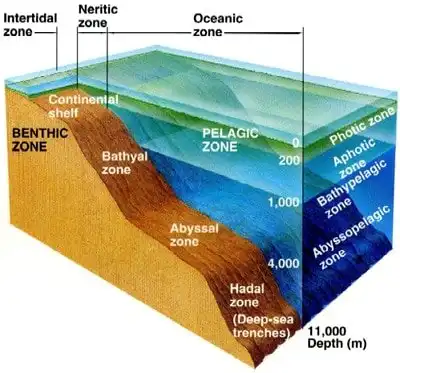
\includegraphics[width=0.8\textwidth]{sea_layers.png}
	\end{center}
	\caption[Petite légende]{Sea layers along depth, from \citep{fig_deep_sea}}
	\label{fig:dsl}
\end{figure}

Despite those extremes conditions, and low rate of food supply deep-sea is far from being lifeless. In fact, deep-sea is considered to be the largest biome of the Earth, and contains 70\% of ocean's microbial cells and 60\% of its heterotrophic activity, playing a crucial role in biogeochemical cycles \citep{salazar2016}. \citet{grassle1992,parkes1994,todo2005} studies shown that life could be found everywhere in the deep-sea, with remarkably high and stable diversity. With first studies launched in the 60's, less that 0.0001\% of the area has been investigated so far \citep{danovaro2017}. Thus, deep-sea remains the most unknown biome of the planet with estimated 10 million species that are yet to discover \citep{danovaro2017,grassle1992}. In particular, data are lacking to evaluate the impact of climate change on the biodiversity of the largest reservoir of biomass, mainly because exploring deep-sea is difficult and requires specific tools, such as rovers \citep{danovaro2008,danovaro2014}. Firstly, deep-sea were regarded as a ore reservoir, where manganese and other metal deposits could be found and extracted, or even as a dumping site for nuclear wastes \citep{baker2020,gillet2013,halfar2002}. But since past decades, capacity of exploration of the deep-sea expanded spectacularly, allowing seachers to discover more about the depth of the oceans \citep{danovaro2014}.
In particular, continental margins, which separates continental shelf from abyssal plains are investigated, because their heterogeneous topography implies varied habitats and hydrodynamics, with impacts on the whole food chain \citep{danovaro2009}. Along continental margins, deep-sea canyons, that incises the edges of continental shelf, appears to be ``biodiversity hotspots'' for pelagic life, in terms of diversity and abundance \citep{aissi2012,danovaro2009,gillet2013,robertson2020}. Because they are the main conduits transfering organic matter and sediments from rich and productive shallow shelf to the low-nutrients deep-sea, canyons constitues peculiar habitats, with evidences of an important biomass and diversity of benthic organisms \citep{canals2006,danovaro2009,leo2012}, but also of fishes assemblages \citep{sion2019,stefanescu1994}. Locally, canyons displays higher nutrients concentrations than in adjacent areas, due to down-welling currents, that makes them favourable habitats for filters and suspension feeders \citep{sion2019}. Abundance of nutrients and preys attracts top predators, some of them being only encountered in those habitats \citep{aissi2012}. Among abundant preys are found euphausiids, shrimps, squids and meso- and bathypelagic fishes \citep{aissi2012,gaskett2001}.

Meso- and bathypelagic fishes are found in every ocean, except Arctic, and are the dominant zooplankton consumers in most oceans, playing a key role in trophic networks \citep{davison2015}~. Living between 200-1000m (mesopelagic) and over 1000m (bathypelagic) deep, those fishes displays very high biomass, mainly carried by Myctophidae family \citep{gaskett2001,kozlov1995,pusch2004}. 

Therefore, 







\subsection{Axes pour une meilleure connaissance de ces écosystèmes}
- comment les espèces se partagent les ressources (bcp d'études déjà terrestres)
         --> focus sur cette communauté particulière qui est pour l'instant peu connue

- 2 approches possibles: 
		- espèce-centrée : seule ou en compétition --> mais limitant pour la comparaison entre écosystèmes différents. 
		- communautaire : certaines espèces sont-elles redondantes ? Plusieurs espèces
occupent la même niche en cas de chevauchement, occupent la même niche fonctionnelle. Se focaliser
sur les fonctions plutôt que sur l'espèce. --> Permet une généralisation de la méthode et une comparaison entre écosystèmes
		- Individus appartenant à la meme niche peuvent être considérés comme appartenant
à la même boîte fonctionelle. 
==> Caractériser un écosystème par les fonctions qu'ils présentent plutôt que par ses espèces

\subsection{Présentation de la démarche et des objectifs}
- mieux connaitre ces communautés à travers les niches qu'elles occupent dans les écosystèmes
- caractériser leurs niches trophiques, comportements, habitats, sensibilité des espèces, 
particularité des espèces, voir les avantages de partager les niches 
- Envisager une approche universelle, permettant la comparaison d'écosystèmes

- Hypothèses: chevauchement de niches entre les espèces, entrainant de la compétition entre les espèces ayant des fonctions similaires, ou ségrégation, où les espèces
utilisent des ressources distinctes et ont des fonctions différentes



\section{Materials \& Methods}
%!TEX root = ./Structure_rapport_final.tex


\subsection{Sampling and specimens}

Fishes were collected during Ifremer's EVHOE (EValuation Halieutique de l'Ouest Européen) research cruises, surveying the Bay of Biscay every fall onboard the \textit{R/V Thalassa}. Several hauls are regularly performed at night to investigate pelagic deep fauna. Each station is precisely defined with its GPS coordinates and located above canyons, at the edge of the continental shelf. 
% Altough they are considered to be ``biodiversity hotspot'', canyons communities are yet relatively unknown, because of the logistic and material difficulties that their exploration implies \citep{gillet2013}.
Pelagic trawling is performed at night, between 700 and 2000 meters, because those fishes perform diel vertical migrations and tend to come closer to the surface at nighttime. To this end, a 25 meters-wide opening trawl is used, with a mesh size decreasing from 76mm to 48mm at the end of the trawl. The trawl-haul duration was 1 hour at 4 kn. 
Once the trawl is pulled back onboard, fishes are sorted, identified up to the species level, and frozen at -20°C. Eleven of the most abundant species in the Bay of Biscay (all teleosts) have been selected for this study. Four of them belong to the Myctophid family (lanternfish), which is the most abundant and widespread family across all oceans \citep{debusserolles2014} and could represent up to 65\% of the pelagic deep-sea biomass \citep{poulsen2013}: \textit{Lampanyctus crocodilus}, \textit{Myctophum punctatum}, \textit{Notoscopelus kroeyeri} and \textit{Ceratoscopelus maderensis}. The second most represented family is the Platytroctidae with two species: \textit{Searsia koefoedi} \& \textit{Normichthys operosus}. This family seems to be found in all oceans but not in the Mediterranean Sea \citep{orrell2016}. Finally, five families are represented by one species each: \textit{Xenodermichthys copei} (Alepocephalidae), \textit{Arctozenus risso} (Paralepididae), \textit{Argyropelecus olfersii} (Sternoptychidae - Hatchetfishes), \textit{Serrivomer beanii} (Serrivomeridae) and \textit{Stomias boa} (Stomiidae) which are common species, found abundantly in every ocean \citep{carvalho1988,froese2019,geidner2008,germain2019}. See \ref{fig:phylotree} for a phylogenetic tree of these species. 


\subsection{Morphological measurements and functional traits}
In the laboratory, the fish were thawed and 24 morphological variables were measured, using an electronic caliper with a precision of 0.01mm. Some of these measurements had previously been recorded by students from La Rochelle University during practical classes in 2018 ($n = 99$), 2019 ($n = 45$), 2020 ($n = 9$) and the rest during this study ($n = 212$). For the sake of statistical robustness and representativity, at least 25 individuals were measured for each species (Table~\ref{table:spcount}).  

%Voir script table_tex.Rnw
\begin{table}[ht]
\centering
\caption[Count, size's mean and range values of species]{Number of individuals measured for each species ($n_1$: previous studies, $n_2$: this study, $n_\text{Tot}$ : $n_1 + n_2$), with their mean standard size and range values in millimeters.}
\label{table:spcount}

\begin{tabular}{rrrrrr}
  \toprule
        &                  &          &       & Mean length & Size range\\ 
Species & $n_1$  & $n_2$ & $n_\text{Tot}$ &   (mm) & (mm) \\ 
  \midrule
  \emph{Lampanyctus crocodilus} &  39 &    &  39 & 107.60 & 73.3 - 146.5 \\ 
  \emph{Xenodermichthys copei} &  38 &    &  38 & 109.68 & 82.3 - 132 \\ 
  \emph{Normichthys operosus} &    &  38 &  38 & 104.69 & 75.64 - 131.62 \\ 
  \emph{Argyropelecus olfersii} &  37 &    &  37 & 56.55 & 32.16 - 89.07 \\ 
  \emph{Notoscopelus kroyeri} &   6 &  30 &  36 & 76.30 & 52.63 - 130.84 \\ 
  \emph{Searsia koefoedi} &   5 &  31 &  36 & 119.94 & 84.8 - 142.75 \\ 
  \emph{Arctozenus risso} &  20 &  10 &  30 & 158.36 & 117.6 - 181.31 \\ 
  \emph{Serrivomer beanii} &    &  30 &  30 & 546.17 & 373 - 879 \\ 
  \emph{Ceratoscopelus maderensis} &    &  30 &  30 & 62.72 & 53.29 - 78.95 \\ 
  \emph{Stomias boa} &    &  26 &  26 & 239.00 & 144 - 311 \\ 
  \emph{Myctophum punctatum} &   8 &  17 &  25 & 65.48 & 52.53 - 80.14 \\ 
  \bottomrule
\end{tabular}
\end{table}

21 functional traits were calculated for each individual from the morphological measurements. They inform on 3 main functions: food acquisition, locomotion and habitat (Table~\ref{table:functraits}).

\begin{sidewaystable}
\centering
\caption[Functional traits descriptions and formulas]{Description and formulas of the functionals traits computed from morphological measurements, following \citep{albouy2011, aneeshkumar2017,boyle2006,brindamour2016,diderich2006,dumay2004,habib2019,ibanez2007,sibbing2000,webb1984,winemiller1991}. Abbreviations used in formulas are provided by raw measurements and detailed in appendices \ref{fig:full_body}, \ref{fig:head} \& \ref{fig:fin}. \texttt{oga}, \texttt{git}, \texttt{pc}, \texttt{pht} are categorial variables directly provided by raw measurements with the first two scores detailed respectively in appendices \ref{fig:git} \& \ref{fig:oga}.}
\label{table:functraits}
\begin{tabular}{>{\bfseries}lll>{\ttfamily}l}
\toprule
Function & Functional trait & Description & Formula  \\ 
\midrule
\multirow{13}{*}{Feeding} &Oral gape axis & Feeding position and depth in the water column & oga \\ 
  &Eye size & Detection of preys and visual acuity for predators & ed/hd \\ 
  &Orbital length & Preys size and behavior (buried, camouflaged) & ed/sl \\ 
  &Oral gape surface & Type and size of preys & mw*md / bw*bd \\ 
  &Oral gape shape & Strategy to capture prey & md/mw \\ 
  &Oral gape position & Fedding position in the water column & mo/hd \\ 
  &Lower jaw length & Compromise between power and opening speed of the mouth & ljl/sl \\ 
  &Gill raker type & Filtration capacities of fish & git \\ 
  &Gill outflow & Succion capacities of fish & ow \\ 
  &Head length & Maximum prey size & hl/sl \\ 
  &Pyloric caeca & Presence/Absence of pyloric caeca & pc \\ 
  &Anus position & Digestive tract length & pal/sl \\ 
\midrule
  \multirow{6}{*}{Locomotion} & Body depth & Swimming capacities of fish linked to their food prospection behavior & bd/sl \\ 
  &Pectoral fin position & Maneuvrability of fish & pfi/pfb \\ 
  &Pectoral fin insertion & Maneuvrability of fish & ppl/sl \\ 
  &Transversal shape & Position in the water column and hydrodynamism & bd/bw \\ 
  &Caudal throttle width & Swimming strategy (cruiser/sprinter) and endurance & cpd \\ 
  &Dorsal fin insertion & Swimming type and behavior & pdl/sl \\ 
\midrule
  \multirow{2}{*}{Habitat} &Eye position & Position in the water column (pelagic/sedentary) & eh/hd \\ 
  &Presence photophores & Presence/Absence of photophores (camouflage, foraging, courtship behavior) & pht \\ 
  &Operculum volume & Filtering capacity and oxygen captation & od/ow \\ 
\bottomrule
\end{tabular}
\end{sidewaystable}

\subsection{Data analysis}
All data analyses were performed using \textsf{R} version 4.0.3 \citep{rcoreteam2021}.

% \textbf{Commentaire : } je vois que tu utilises \verb;\texttsc{}; quand tu parles de tes mesures et des traits. Attention, je crois que le Times New Roman ne dispose pas de cette police spéciale qui fait des "Petites majuscules". Du coup, la commande n'a aucun effet. J'ai donc remplacé par \verb;\texttt; partout où je l'ai trouvé ! D'ailleurs, utilises aussi plutôt ça plutôt que l'italique pour les noms de logiciels, de packages, etc.

\subsubsection{Data pre-processing}
Because measurements came from several observers, raw data had to be checked for outliers. To do so, all values (except the standard length \texttt{sl}) were standardized by \texttt{sl} and the interquartile range (IQR) method of outlier detection was applied to remove outliers. According to this method, for each measurement and species, outliers are defined as every value outside this interval: 
\begin{center}
$ [Q1 - 1.5 \times IQR, Q3 + 1.5 \times IQR]$ \\
with $Q1$ and $Q3$ being respectively the first and third quartile, and $IQR = Q3 - Q1$. 
\end{center}{}

Missing values initially present in the dataset ($n = 52$) and induced by the outlier removal function ($n = 307$), were then imputed using the $k$-Nearest Neighbor (kNN) algorithm. Suppose that the individual $i$ has a missing value $X_i$ for the variable $X$. The algorithm identifies the $k$ nearest neighbors of $i$ based on all available variables (\emph{i.e.} all variables but $X$). The values of $X$ observed in the $k$ nearest neighbors of $i$ are then used to infer $X_i$ using Euclidean distances between $i$ and its $k$ nearest neighbors. The computations were performed by the \texttt{step\_knnimpute()} function from the \texttt{tidymodels} R package \citep{kuhn2020}, with a number of nearest neighbors of $k = \sqrt{N}$, with $N$ being the number of individuals for each species. The accuracy of the imputation was then checked with a linear regression of each variable with respect to \texttt{sl}. From this cleaned dataset, the functional traits were computed using formulas in Table~\ref{table:functraits}. 

\subsubsection{Factorial Analysis of Mixed Data (FAMD)}

To assess the similarities or differences of traits in species, a Factor Analysis of Mixed Data (FAMD) was performed using the \texttt{FactoMineR} package. This type of multivariate analysis is suited for datasets containing a mix of qualitative and quantitative variables. It performs a Principal Component Analysis (PCA) on quantitative variables and a Multiple Correspondence Analysis (MCA) on qualitative variables. The results of an FAMD are interpreted in the same way as those of a PCA: both methods are used to assess (i) similarities and differences among individuals and (ii) to check for associations between variables. Because \textit{Serrivomer beanii} does not have pectoral nor pelvic fins, and because this analysis can not handle missing values, zero values were attributed for \texttt{PFB}, \texttt{PFI}, \texttt{PPL} and \texttt{PVL}. Because of this specific particularity, complementarty analysis was run. First, the same FAMD analysis was run without \textit{S. beanii}, to assess the discrimination between all remaining species. Then, the analysis was run with all species (including \emph{S. beanii}) but without the traits missing for \emph{S. beanii} (\emph{i.e.} \texttt{PFB}, \texttt{PFI}, \texttt{PPL} and \texttt{PVL}), to verify that the observed differences were not exclusively dependants on these traits. The categorical variables were managed as follow: scores were used for both oral gape axis and gill raker type (see Figures~\ref{fig:oga} and \ref{fig:git}), whereas pyloric caeca and photophores were binary defined (0 = absent, 1 = present). For each principal component (PC), all traits that have a contribution greater than or equal to a threshold $t$ are considered relevant (with $t = 100 / \text{number of variables}$). Here, 21 functional traits were computed, meaning that $t \approx 4.8$. On the resulting FAMD graph, we added 95\% confidence interval ellipses representing the functional niche of each species. These ellipses assume a multinormal distribution of the functional traits.

 \subsection{Functional niche analysis}
 The coordinates of individuals projected on the FAMD axes were used to compute (i) the surface of the functional niche of each species, and the overlap of niches for all possible pairs of species. This analysis was only run on the first two factorial axes (PCs), because they are the ones carrying most of the information about the community's structure. The method used here is similar to isotopic niche analysis, which is much more documented. We used the \texttt{SIBER} package (Stable Isotope Bayesian Ellispes in R) and adapted it to our purpose \citep{siber2011}. For each species the ellipse surface was computed, and the overlap of ellipses between all pairs of species was assessed with the \texttt{maxLikeOverlap()} function. Absolute niche surfaces were then standardized by the smallest niche, to facilitate the comparison of relative differences in niche sizes. The relative overlap was assessed as the ratio of the overlap value to the size of the niche, for each species of each pair. Finally, the total overlap for a pair of species was determined by dividing the overlap value by the sum of the area of the niches of the two species. In order to assess the sensitivity of the method to insufficient sample size, niche surfaces were also computed for various sample sizes ($n$) following a bootstrap procedure. To this end, between 100 to $10\,000$ individuals from our dataset were sampled at random, and area of all niche's was recalculated $10\,000$ times.

 Functional niches were further investigated using the \texttt{funrar} R package, to compute functional rarity \citep{matthiasgrenie2017}. Based on indices characterizing the rarity of functions within a system \citep{violle2017}, the aim is to assess the local functional diversity of the traits in our dataset. First a distance matrix is computed using Gower's distance as it can deal with both quantitatives and qualitatives variables \citep{brindamour2016,matthiasgrenie2017}. Then, the \texttt{distinctiveness\_global()} function is applied to measure how functionnally rare a species is, compared to other species of the community. Distinctiveness results range from 0 (no distinctiveness) to 1, when a species is, locally and/or functionnally, different from the others \citep{matthiasgrenie2017}.

 \subsection{Kernel density estimation}
 When two or more niches overlap, it is interesting to detail which traits are most similar between species. To this end, we used a parametric kernel density function \citep{mouillot2005} , which has been used in a similar context by \citet{aneeshkumar2017}. Along a trait axis, the function returns the overlap value between $N$ overlapping species, ranging from 0 (no overlap) to 1 ($N$ species have identical, fully overlapping densities).
\section{Results}
%!TEX root = ./Structure_rapport_final.tex

\subsection{Factorial Analysis of Mixed Data}

The first 5 axis FAMD components explained 78.9\% of the total variation (Table \ref{table:cont_abs}). The first axis (30.6\% of explained variance) is strongly correlated with food acquisition with traits such as \emph{body depth} (a = 12.8), \emph{oral gape axis} (a=11.9), \emph{gill raker type} (a = 11.9), \emph{lower jaw length} (a=10.4) and oral gape surface (a=9.91) (Table \ref{table:cont_abs}). Along this axis, all traits have increasing values toward the right (see \ref{fig:corr_circ_12} for details). As can be seen on Figure \ref{fig:famd12}, this axis clearly separates 3 groups of fishes. At the left, fishes have a low transversal shape (meaning that both \textsc{bd} and \textsc{bw} have similar values, consistent with an elongated body), short lower jaw and small oral gape surface, such as \textit{A. risso}, \textit{S. boa} and \textit{S. beanii}. On the right of this axis, fishes display high body depth values suggesting a laterally compressed form, such as \textit{A. olfersii}. 
The second axis (17.7\% of explained variance) is correlated with food prospection behaviour, through locomotion with \emph{pectoral fin insertion} (a = 15.0), \emph{pectoral fin position} (a = 12.7), which are anti-correlated (see Figure \ref{fig:corr_circ_12}) and diet through \emph{anus position} (a = 10.52) and \emph{oral gape shape} (a = 8.67) (Table \ref{table:cont_abs}). This axis separates the 3 species on the left, \textit{A. risso} diplay higher values of pectoral fin insertion, meaning that the fin is inserted further on the body than \textit{S. boa}, while the fin position on the body depth is lower. Because \textit{S. beanii} does not have pectoral fin, same analysis has been run without traits refering to pectoral or pelvic fins to look if discrimination between species were highly dependant if these traits. Same results than Figure \ref{fig:famd12} were obtained, with \textit{S. boa} and \textit{S. beanii} slightly overlapping. 
The third axis (explaining 13.1\% of total variance) mainly carries traits linked to the habitat and predatory behavior, with strong influence of \emph{oral gape axis} (a = 23.3), \emph{gill raker type} (a = 23.3), \emph{presence of photophores} (a = 11.2) and \emph{caudal throttle width} (a = 10.1) (Table \ref{table:cont_abs}). On the left of this axis (see Figure \ref{fig:famd34}), species are characterized by wide caudal throttle, supra-terminal oral gape axis and `C' gill rakers type (see \ref{fig:oga}), whereas species on the right have a superior oral gape axis and `A' type of gill rakers (see Figure \ref{fig:corr_circ_34}).
+ INTERPRETATION DE L'AXE 4 : operculum volume, anus position, dorsal fin and pyloric caeca --> peut-être en lien avec un comportement de prédateur ou de digestion de proies difficiles ?  

% Table of contributions of variables for 5 first axis
\begin{table}[ht]
\centering
\label{table:cont_abs}
\caption{Correlation bewteen 5 first PC's component and functional traits. In bold, correlations higher than threshold (4.8)}
\begin{adjustbox}{max width=1.1\textwidth,center}
\begin{tabular}{rrrrrr}
  \hline
 & PC1 & PC2 & PC3 & PC4 & PC5 \\ 
  \hline
Eye size & 3.60 & \textbf{8.20} & 2.12 & \textbf{5.14} & 0.80 \\ 
  Orbital length & \textbf{6.03} & \textbf{5.95} & 2.38 & 0.17 & 0.42 \\ 
  Oral gape surface & \textbf{9.91} & 0.32 & 1.16 & 0.60 & 1.56 \\ 
  Oral gape shape & 0.66 & \textbf{8.67} & 1.72 & 3.05 & 3.59 \\ 
  Oral gape position & 0.85 & 1.22 & 0.41 & 4.02 & 0.02 \\ 
  Lower jaw length & \textbf{10.44} & 0.76 & 1.20 & 0.00 & \textbf{5.17} \\ 
  Gill outflow & \textbf{5.82} & 0.01 & 0.00 & 2.21 & \textbf{15.16} \\ 
  Operculum volume & 1.98 & 1.74 & 0.61 & \textbf{18.40} & 4.80 \\ 
  Head length & \textbf{5.00} & \textbf{7.12} & 3.72 & 3.81 & 4.15 \\ 
  Anus position & 0.03 & \textbf{10.52} & 1.81 & \textbf{20.99} & 0.19 \\ 
  Body depth & \textbf{12.80} & 0.25 & 0.35 & 0.06 & 0.10 \\ 
  Pectoral fin position & 0.83 & \textbf{12.72} & 0.00 & \textbf{11.69} & 4.20 \\ 
  Pectoral fin insertion & 1.84 & \textbf{14.96} & \textbf{5.84} & 0.03 & 0.58 \\ 
  Transversal shape & \textbf{8.68} & 0.10 & \textbf{6.30} & 0.48 & 0.00 \\ 
  Caudal throttle width & 1.66 & 3.20 & \textbf{10.09} & 0.18 & \textbf{6.07} \\ 
  Dorsal fin insertion & 3.03 & 4.37 & 0.32 & \textbf{18.04} & \textbf{6.03} \\ 
  Eye position & 0.96 & 3.42 & 3.82 & 0.19 & 3.56 \\ 
  Oral gape axis & \textbf{11.88} & 4.72 & \textbf{23.29} & 0.44 & \textbf{4.86} \\
  Gill raker type & \textbf{11.88} & 4.72 & \textbf{23.29} & 0.44 & \textbf{4.86} \\ 
  Pyloric caeca & 0.34 & 1.27 & 0.42 & \textbf{5.13} & \textbf{26.98} \\ 
  Presence of photophores & 1.82 & \textbf{5.74} & \textbf{11.17} & \textbf{4.92} & \textbf{6.90} \\ 
   \hline
\end{tabular}
\end{adjustbox}
\end{table}

% Or relative values ?
% \begin{table}[ht]
% \centering
% \label{table:cont_abs}
% \caption{Correlation bewteen 5th first PC component and functional traits. In bold, correlations higher than threshold (?????????}
% \begin{adjustbox}{max width=1.1\textwidth,center}
% \begin{tabular}{rrrrrr}
%   \hline
%  & PC1 & PC2 & PC3 & PC4 & PC5 \\ 
%   \hline
% Eye\_size & 0.06 & 0.11 & 0.00 & 0.01 & 0.00 \\ 
%   Orbital\_length & 0.18 & 0.06 & 0.00 & 0.00 & 0.00 \\ 
%   Oral\_gape\_surface & 0.49 & 0.00 & 0.00 & 0.00 & 0.00 \\ 
%   Oral\_gape\_shape & 0.00 & 0.12 & 0.00 & 0.00 & 0.00 \\ 
%   Oral\_gape\_position & 0.00 & 0.00 & 0.00 & 0.01 & 0.00 \\ 
%   Lower\_jaw\_length & 0.54 & 0.00 & 0.00 & 0.00 & 0.01 \\ 
%   Gill\_outflow & 0.17 & 0.00 & 0.00 & 0.00 & 0.08 \\ 
%   Operculum\_volume & 0.02 & 0.00 & 0.00 & 0.15 & 0.01 \\ 
%   Head\_length & 0.12 & 0.08 & 0.01 & 0.01 & 0.01 \\ 
%   Anus\_position & 0.00 & 0.18 & 0.00 & 0.20 & 0.00 \\ 
%   Body\_depth & 0.  & 0.00 & 0.00 & 0.00 & 0.00 \\ 
%   Pectoral\_fin\_position & 0.00 & 0.27 & 0.00 & 0.06 & 0.01 \\ 
%   Pectoral\_fin\_insertion & 0.02 & 0.37 & 0.03 & 0.00 & 0.00 \\ 
%   Transversal\_shape & 0.37 & 0.00 & 0.04 & 0.00 & 0.00 \\ 
%   Caudal\_throttle\_width & 0.01 & 0.02 & 0.09 & 0.00 & 0.01 \\ 
%   Dorsal\_fin\_insertion & 0.04 & 0.03 & 0.00 & 0.15 & 0.01 \\ 
%   Eye\_position & 0.00 & 0.02 & 0.01 & 0.00 & 0.00 \\ 
%   Oral\_gape\_axis & 0.35 & 0.02 & 0.25 & 0.00 & 0.00 \\ 
%   Gill\_raker\_type & 0.35 & 0.02 & 0.25 & 0.00 & 0.00 \\ 
%   Pyloric\_caeca & 0.00 & 0.00 & 0.00 & 0.01 & 0.26 \\ 
%   Presence\_photophores & 0.02 & 0.06 & 0.11 & 0.01 & 0.02 \\ 
%    \hline
% \end{tabular}
% \end{adjustbox}
% \end{table}

% Plot of FAMD axis 1 and 2
\begin{figure} [!htbp]
	\begin{center}
		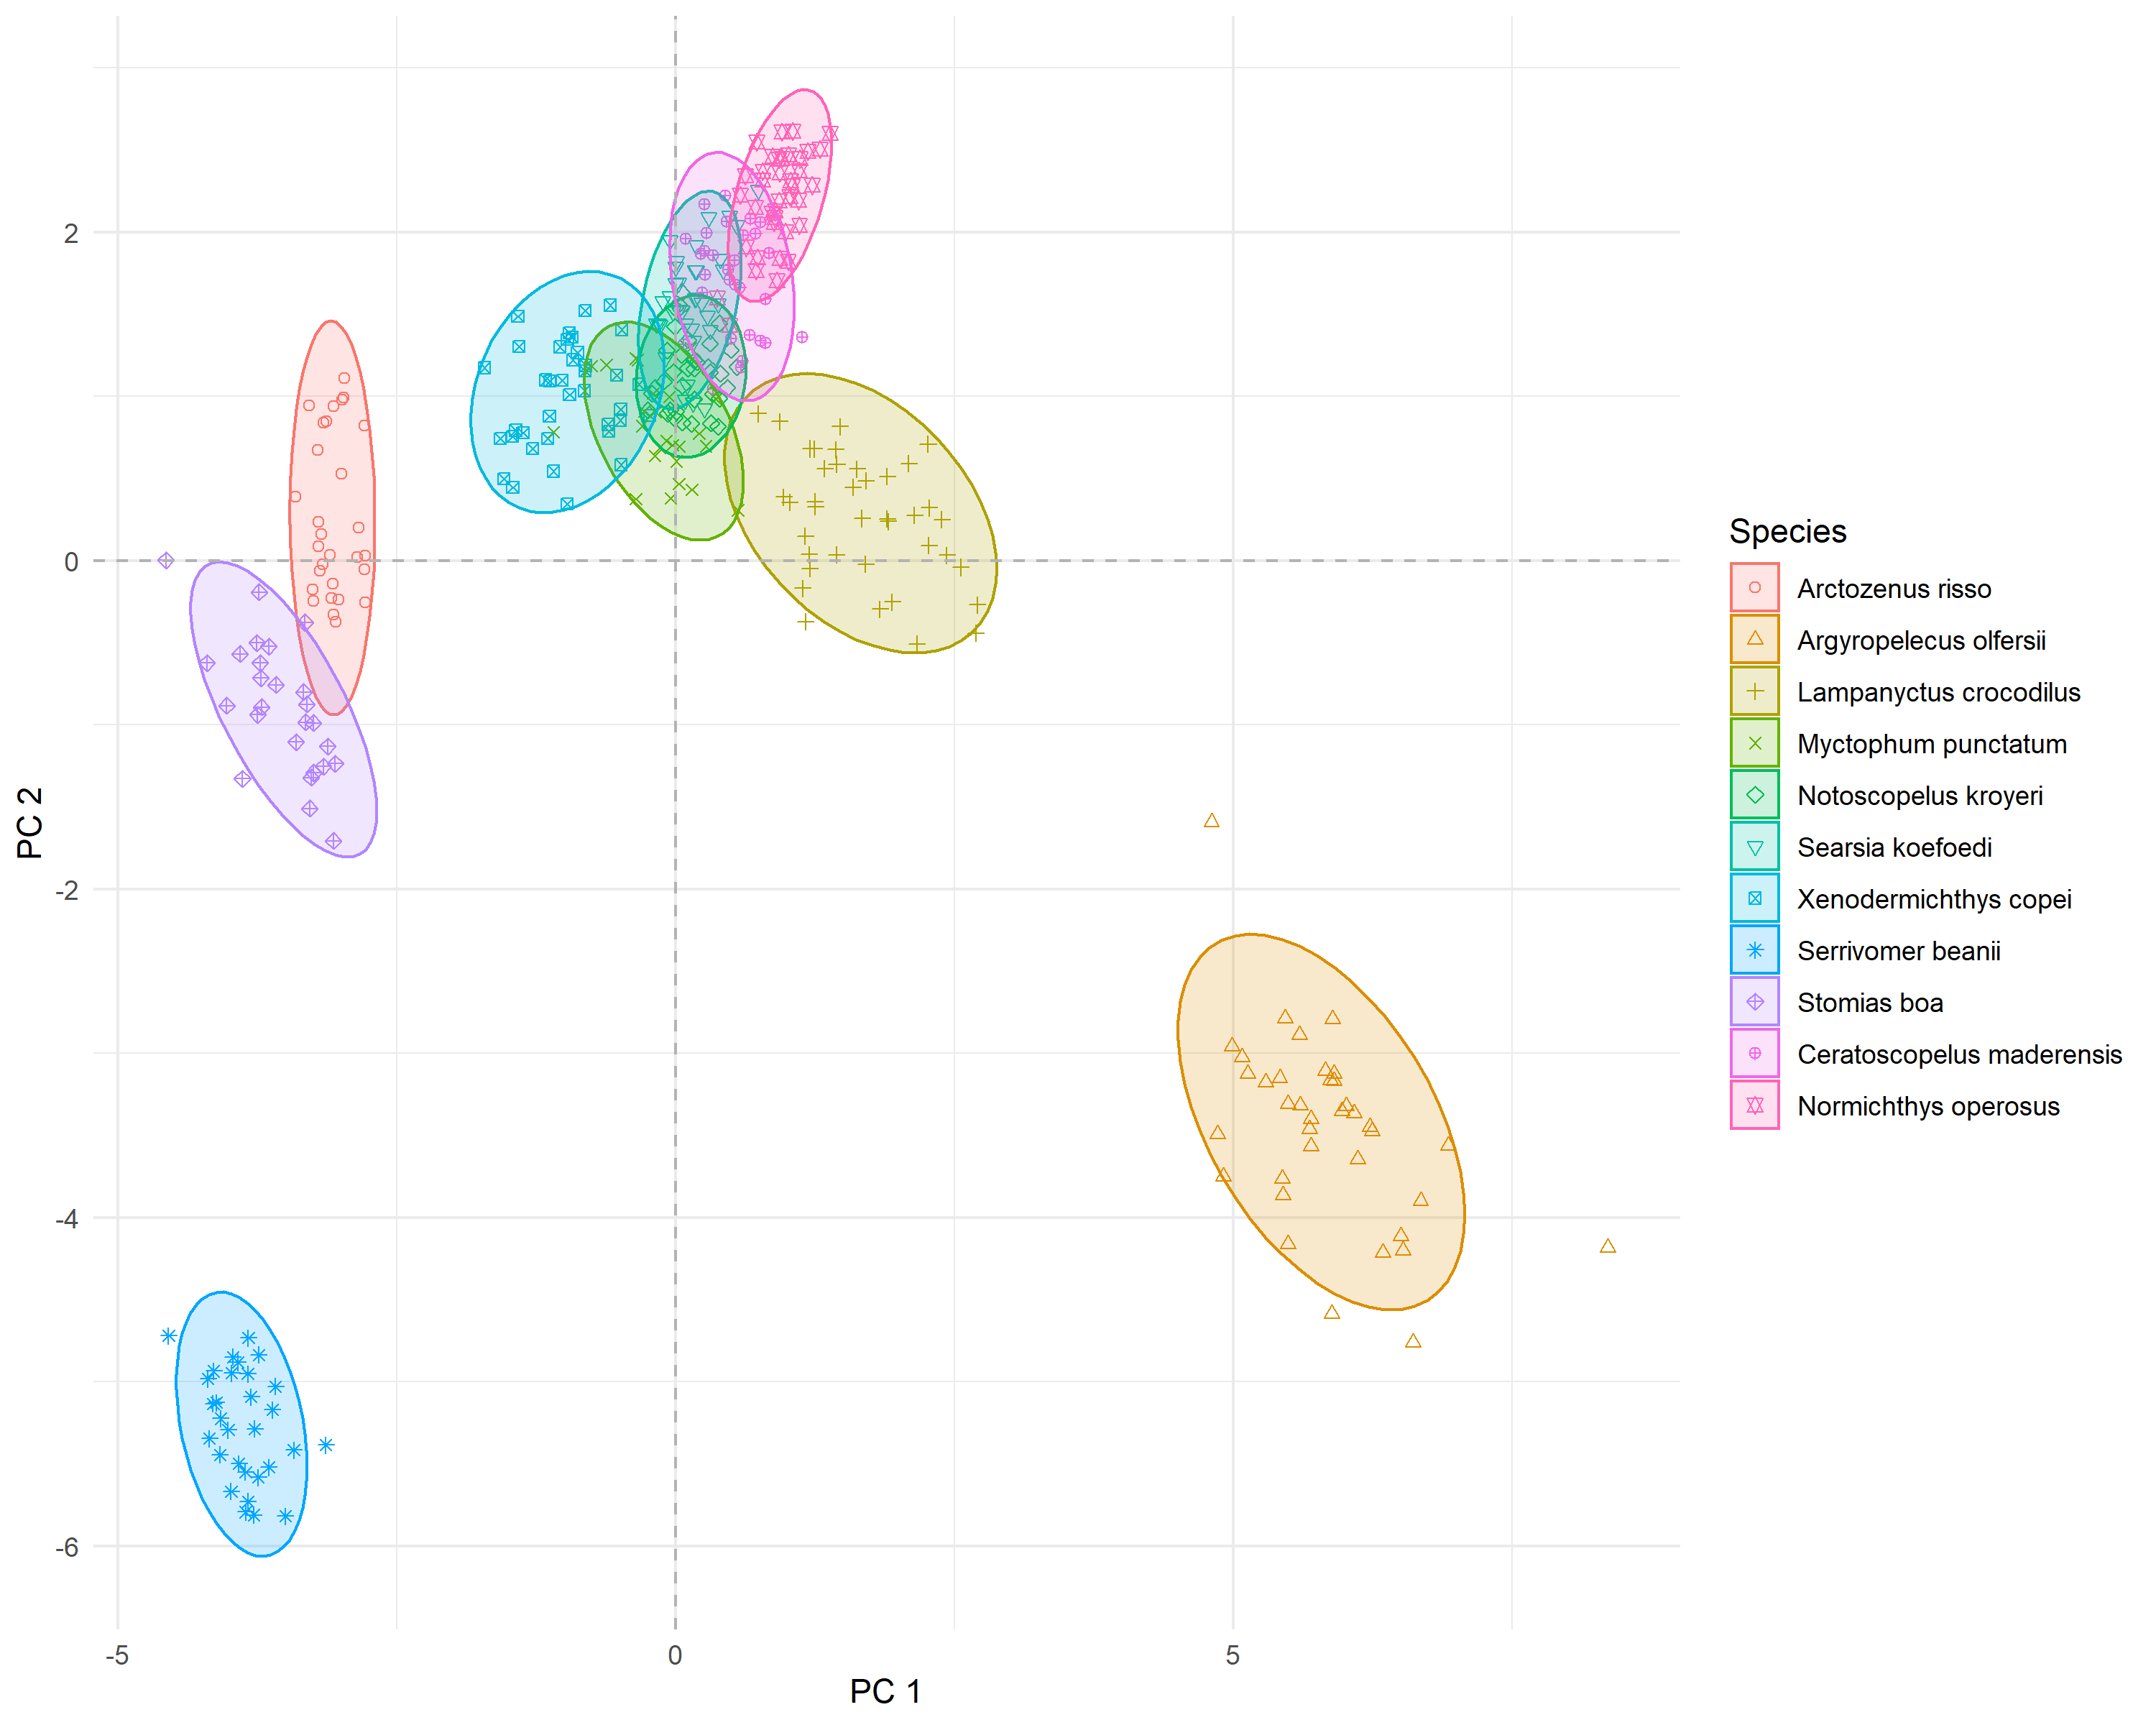
\includegraphics[width=\textwidth]{FAMD_1_2.png}
	\end{center}
	\caption{FAMD results for PC 1 and 2.}
	\label{fig:famd12}
\end{figure}

% Plot of FAMD axis 3 and 4
\begin{figure} [!htbp]
	\begin{center}
		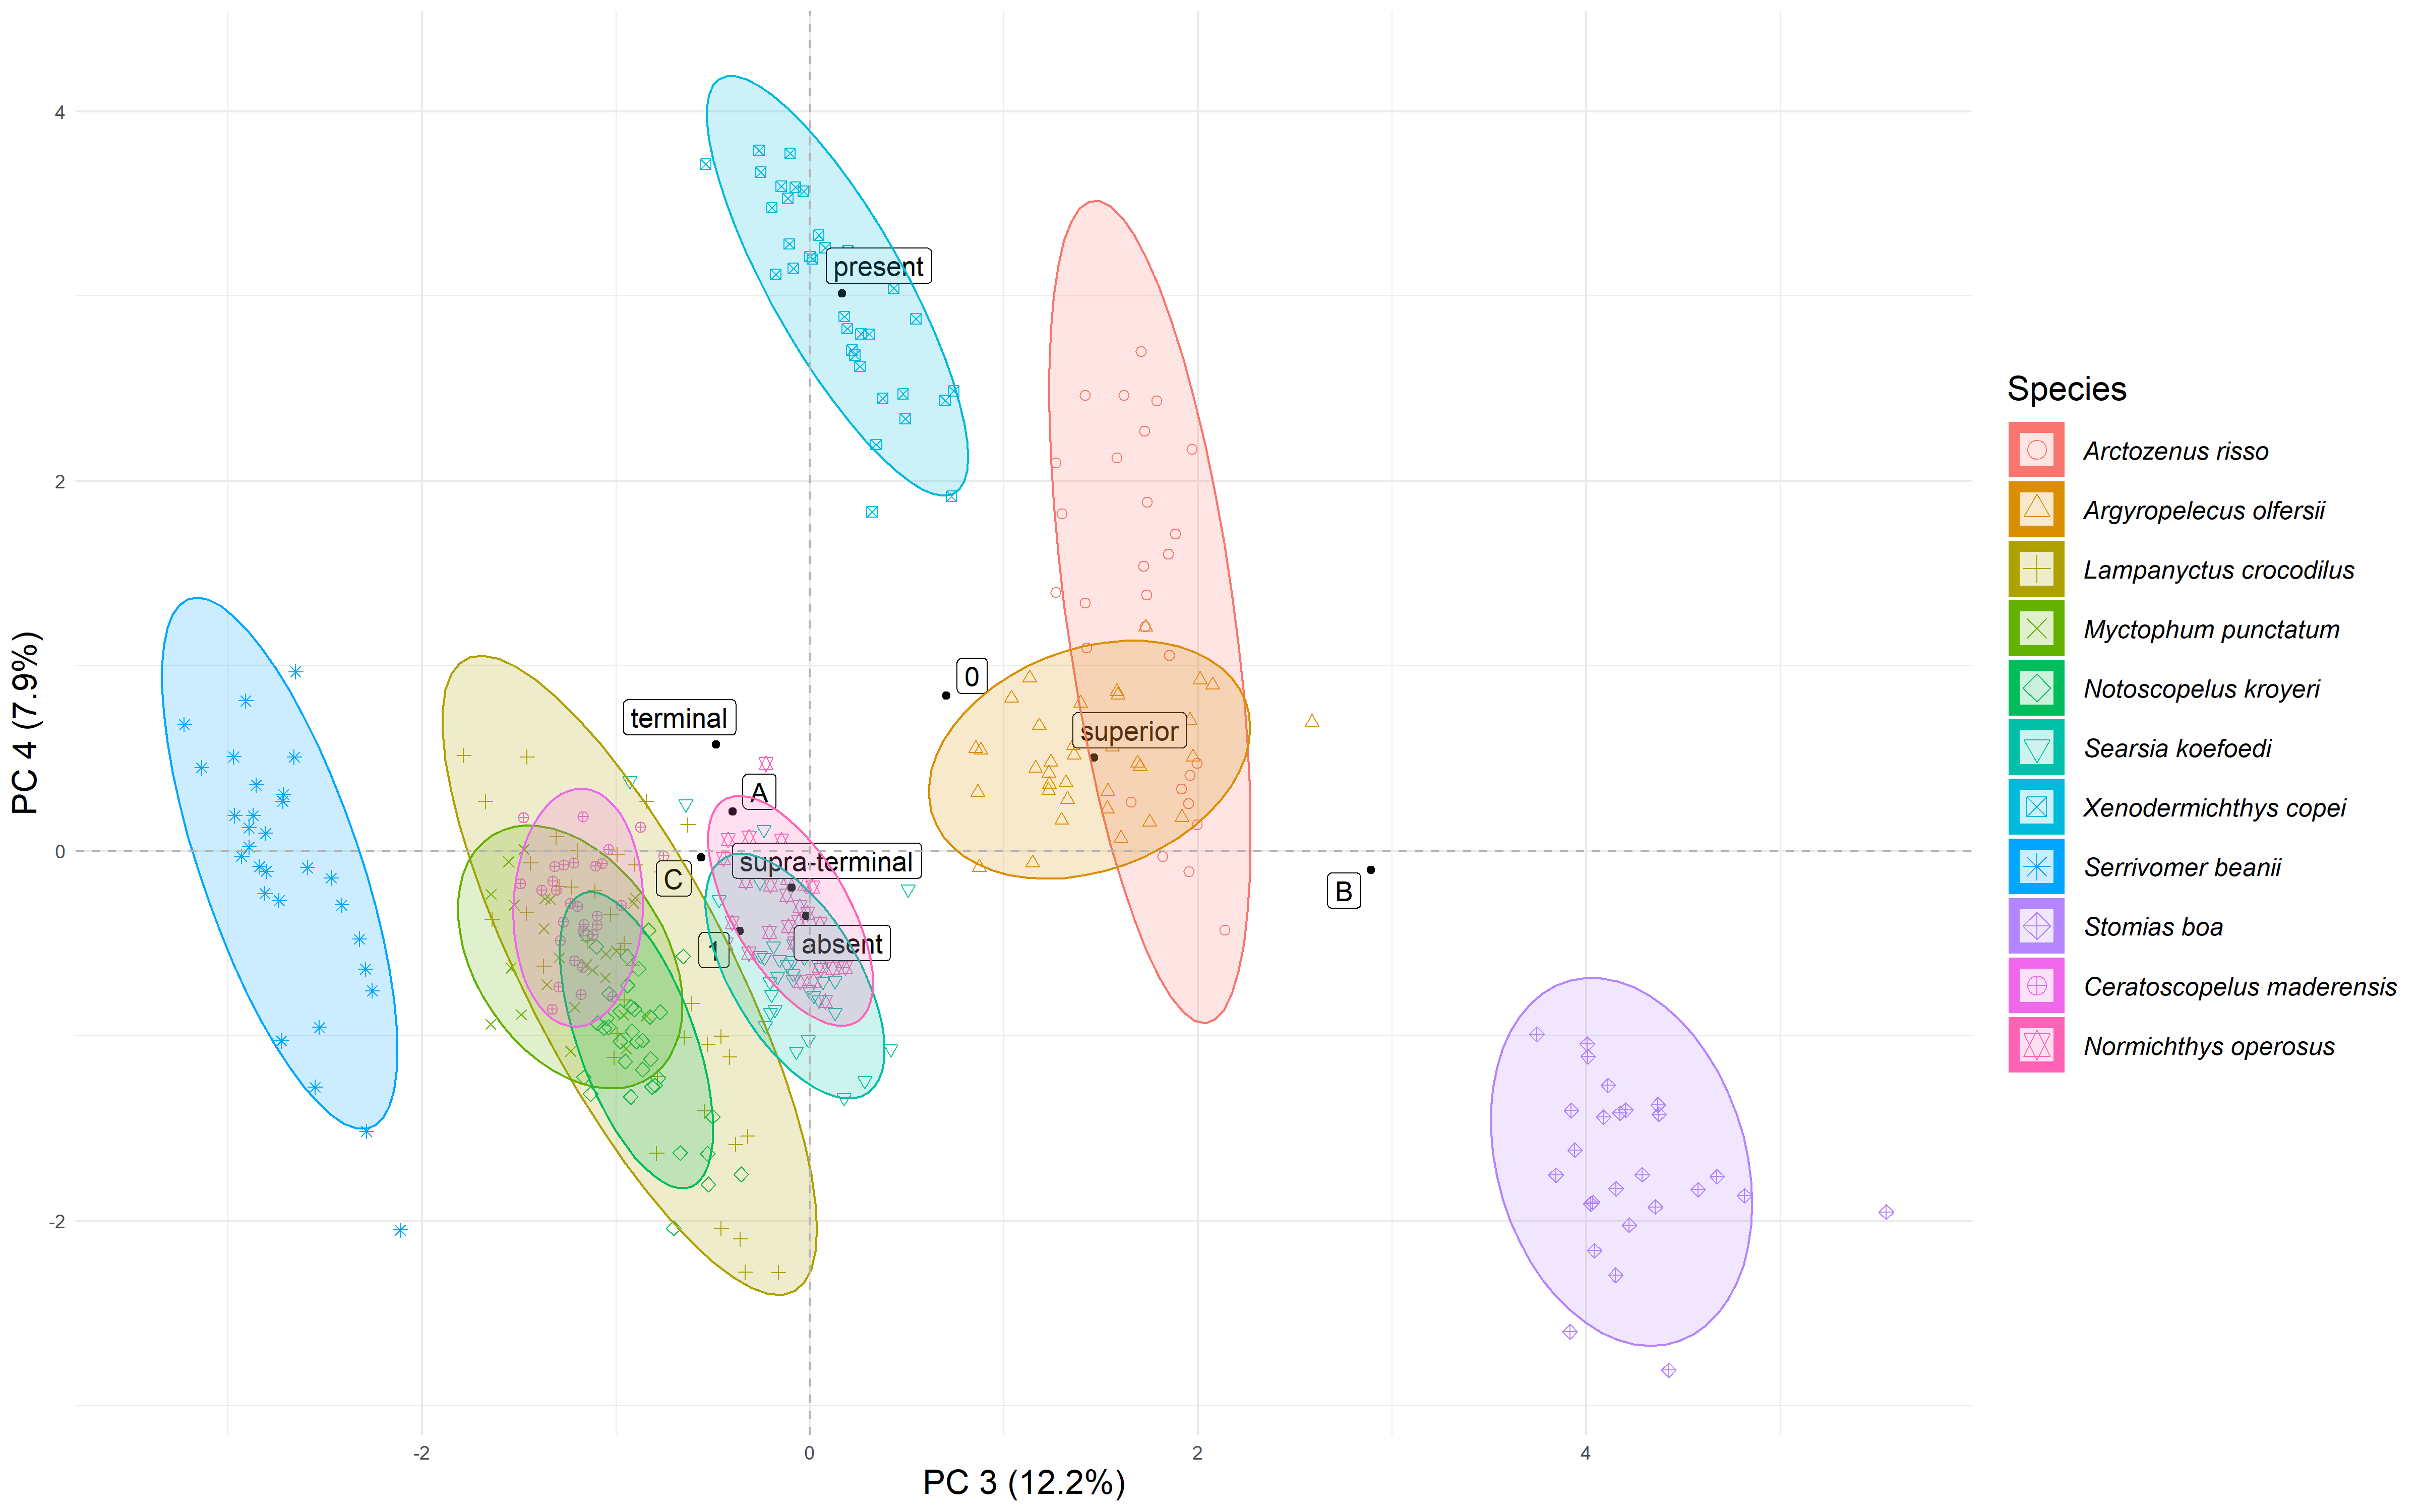
\includegraphics[width=\textwidth]{FAMD_3_4.png}
	\end{center}
	\caption{FAMD results for PC 3 and 4.}
	\label{fig:famd34}
\end{figure}


\subsection{Functional niche area and overlap}

As can be seen on both \ref{fig:famd12} and \ref{fig:famd34}, 6 species present overlapping on the 4 first most discriminant axis, meaning that they are likely to be very much alike. 

% Niche standardardised areas
\begin{table}[ht]
\centering
\label{table:sp_area}
\caption{Standardized area of functional niches.}
\begin{adjustbox}{max width=1.1\textwidth,center}
\begin{tabular}{lr}
  \hline
Species & Area \\ 
  \hline
Argyropelecus olfersii & 5.30 \\ 
  Lampanyctus crocodilus & 3.20 \\ 
  Stomias boa & 2.33 \\ 
  Xenodermichthys copei & 2.14 \\ 
  Arctozenus risso & 2.03 \\ 
  Myctophum punctatum & 1.83 \\ 
  Ceratoscopelus maderensis & 1.80 \\ 
  Serrivomer beanii & 1.73 \\ 
  Searsia koefoedi & 1.10 \\ 
  Normichthys operosus & 1.02 \\ 
  Notoscopelus kroyeri & 1.00 \\ 
   \hline
\end{tabular}
\end{adjustbox}
\end{table}


% Niche overlap 
PROBLEME CHIFFRE SIGNIF.

\begin{table}[ht]
\centering
\label{table:ell_ovlp}
\caption{Species niche overlap}
\begin{adjustbox}{max width=1.1\textwidth,center}
\begin{tabular}{llrrr}
  \hline
Species1 & Species2 & Overlap of Species 2 over Species 1 (\%) & Overlap of Species 1 over Species 2 (\%) & Total overlap (\%)\\ 
  \hline
Notoscopelus kroyeri & Searsia koefoedi & 62.20 & 56.49 & 29.60 \\ 
  Searsia koefoedi & Ceratoscopelus maderensis & 70.63 & 43.30 & 26.84 \\ 
  Myctophum punctatum & Notoscopelus kroyeri & 41.31 & 75.60 & 26.71 \\ 
  Ceratoscopelus maderensis & Normichthys operosus & 29.57 & 51.99 & 18.85 \\ 
  Notoscopelus kroyeri & Ceratoscopelus maderensis & 43.63 & 24.29 & 15.60 \\ 
  Myctophum punctatum & Searsia koefoedi & 22.35 & 37.14 & 13.95 \\ 
  Searsia koefoedi & Normichthys operosus & 15.75 & 16.98 & 8.17 \\ 
  Xenodermichthys copei & Ceratoscopelus maderensis & 13.84 & 16.48 & 7.52 \\ 
  Myctophum punctatum & Ceratoscopelus maderensis & 12.30 & 12.53 & 6.21 \\ 
  Lampanyctus crocodilus & Myctophum punctatum & 8.04 & 14.06 & 5.11 \\ 
  Searsia koefoedi & Xenodermichthys copei & 8.56 & 4.41 & 2.91 \\ 
  Lampanyctus crocodilus & Ceratoscopelus maderensis & 4.51 & 8.04 & 2.89 \\ 
  Lampanyctus crocodilus & Notoscopelus kroyeri & 2.94 & 9.41 & 2.24 \\ 
  Notoscopelus kroyeri & Normichthys operosus & 0.62 & 0.61 & 0.31 \\ 
   \hline
\end{tabular}
\end{adjustbox}
\end{table}


\subsection{Kernel density estimation}
% Plot of density kernel
The estimation of kernel density overlap for functional traits of overlapping species concludes that these species are all overlaping for 11 traits (see figure \ref{fig:dpo}). The overlap is maximum for the position of the oral gape (trait n°5) with an overlap value of 0.338. This means that, along this functional trait, these 6 species share nearly 34\% of their density. Species also share nearly 25\% and 29\% of their density when looking at body depth (trait n°11) and eye position (trait n°17, respectively. Finally, lower jaw length (trait n°6) and pectoral fin position (trait n°12) values also seem to be common to those species, with 16\% and 19\% of density shared, respectively. To a lesser extent, species share 12\% of the eye size values (trait n°2).

\begin{figure} [!htbp]
	\begin{center}
		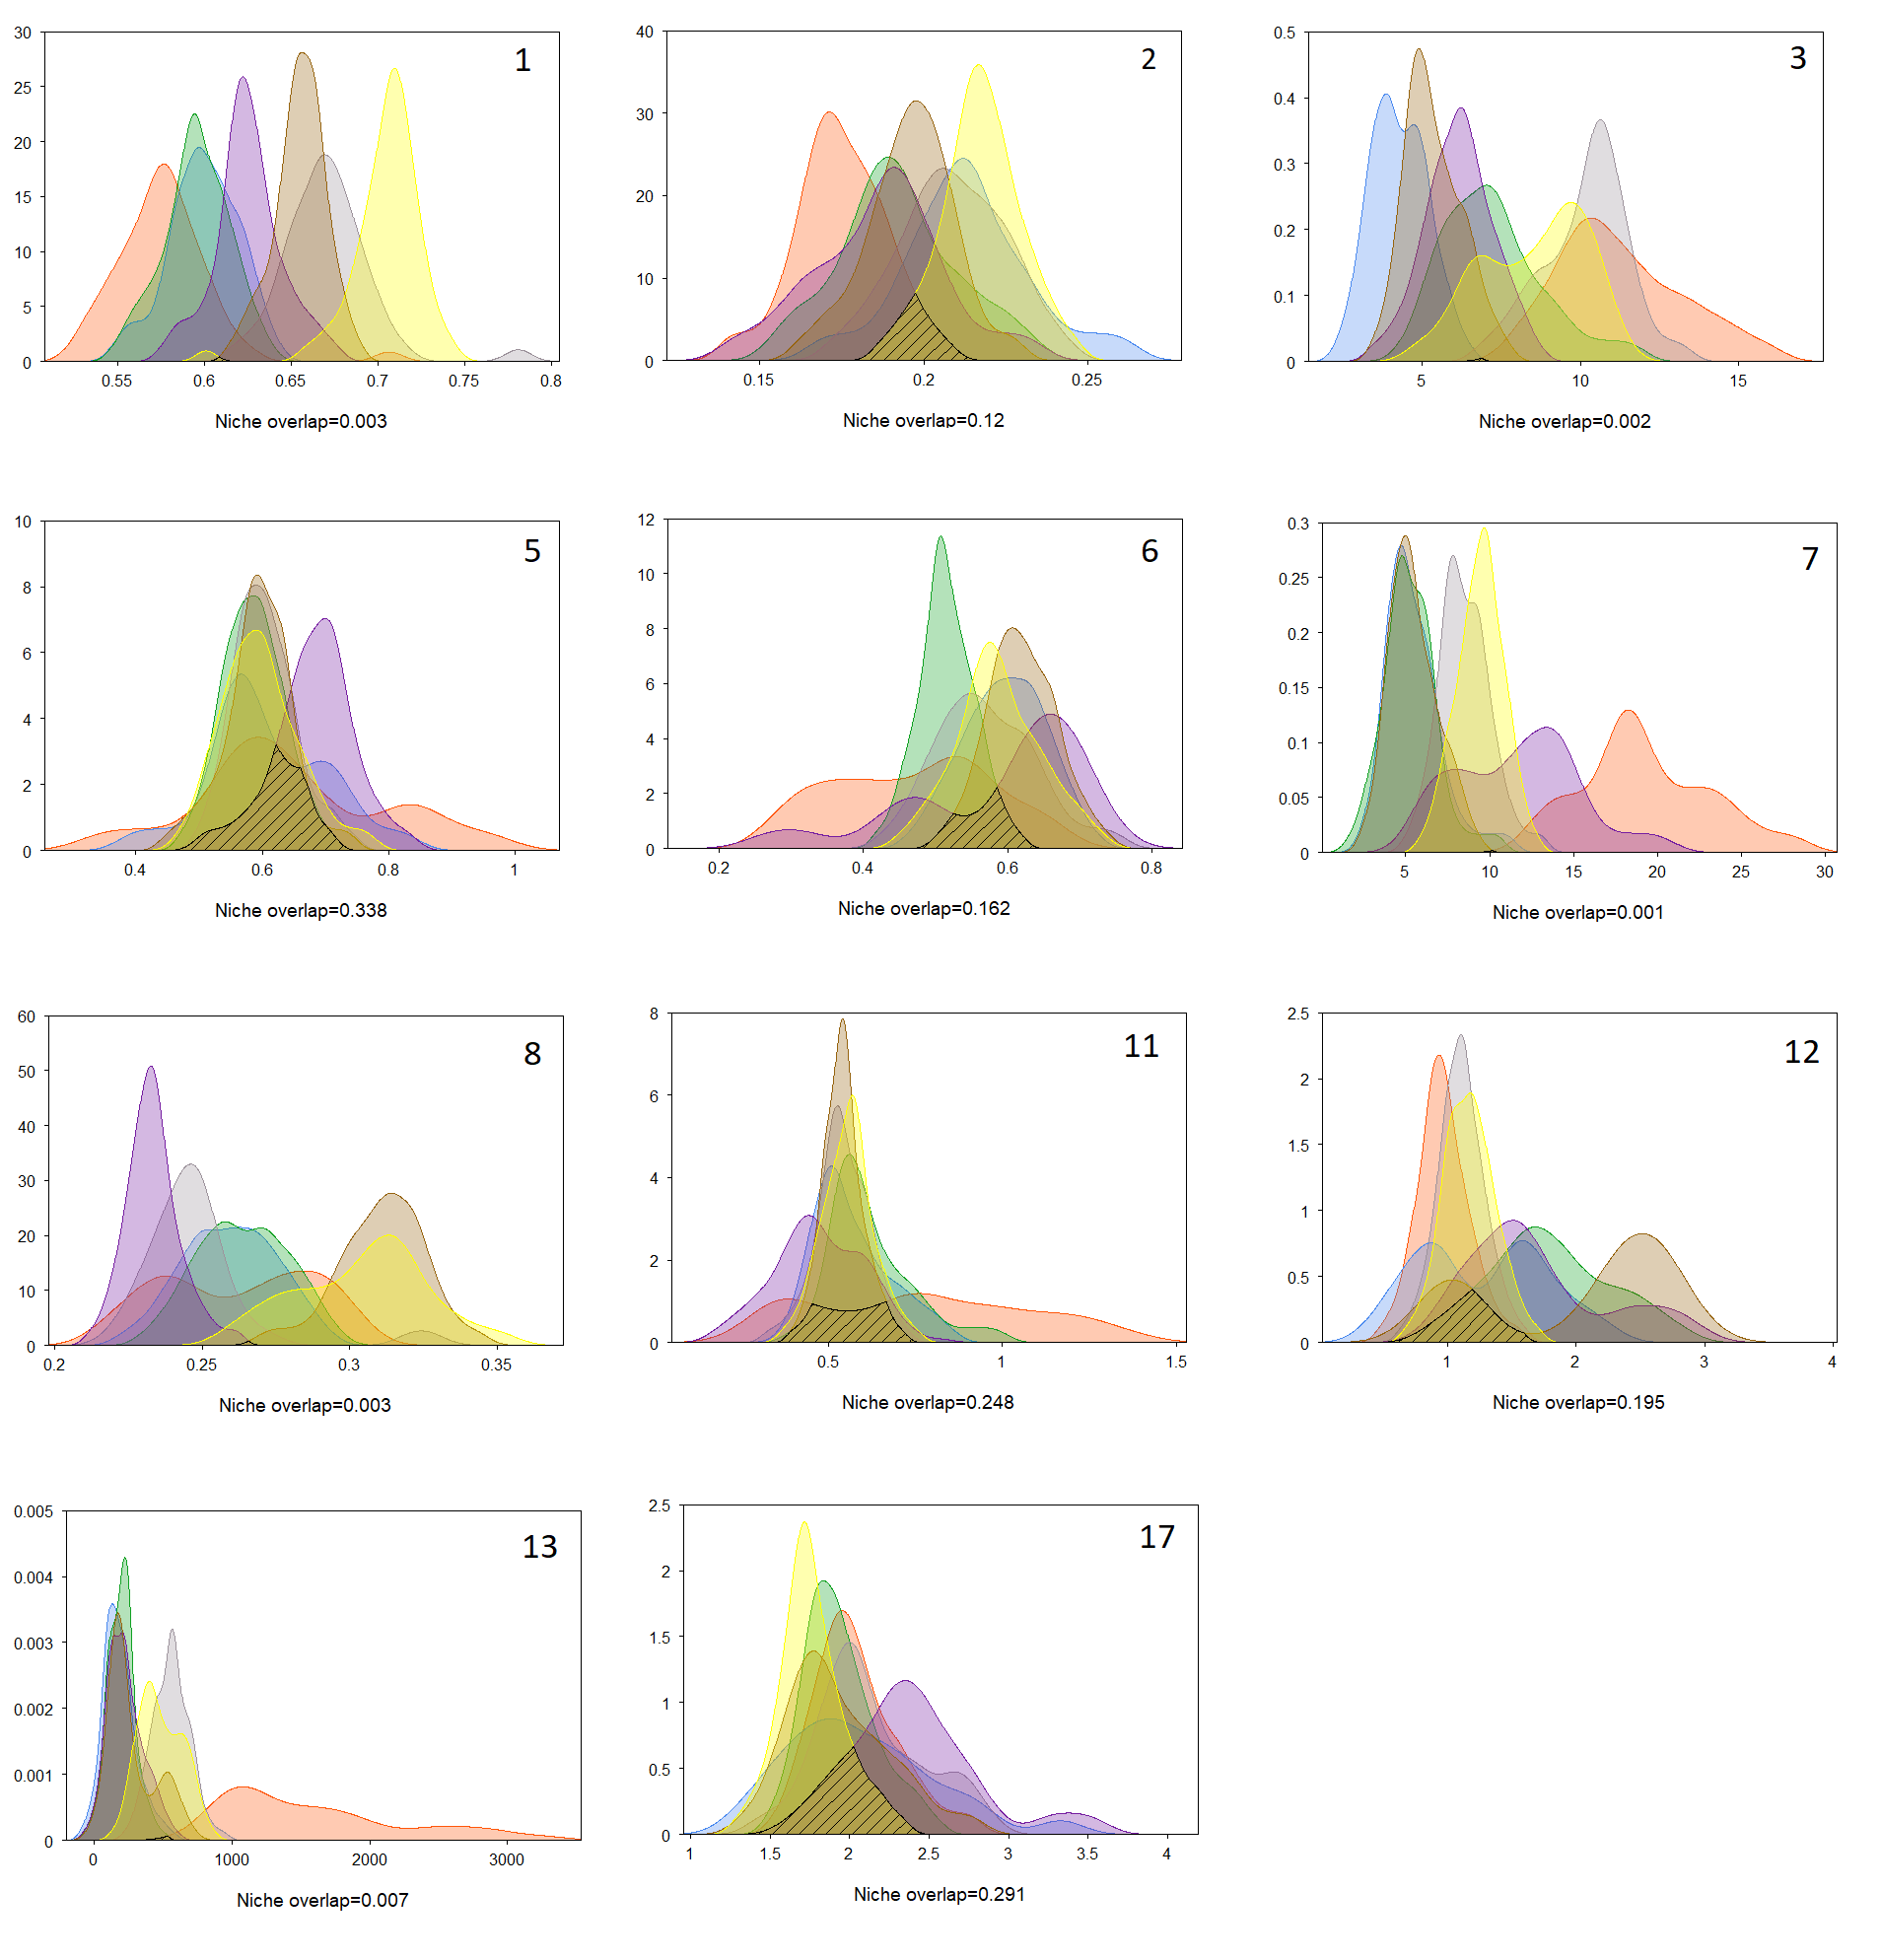
\includegraphics[width=\textwidth]{Density_plot.png}
	\end{center}
	\caption{Kernel density overlap for 11 functional traits and overlaping species. Colors correspond to following species: orange - \textit{L. crocodilus}; brown - \textit{C. maderensis}; yellow - \textit{N. operosus}; purple - \textit{X. copei}; green - \textit{N. kroyeri}; blue - \textit{M. punctatum}.}
	\label{fig:dpo}
\end{figure}
% \section{Discussion}
% \section{Conclusion}

\appendix
%!TEX root = ./Structure_rapport_final.tex

\renewcommand\thefigure{\thesection.\arabic{figure}}
\setcounter{figure}{0}

% \section{Phylogenetic tree}
% Phylotree used in MM
\begin{figure} [!htbp]
	\begin{center}
		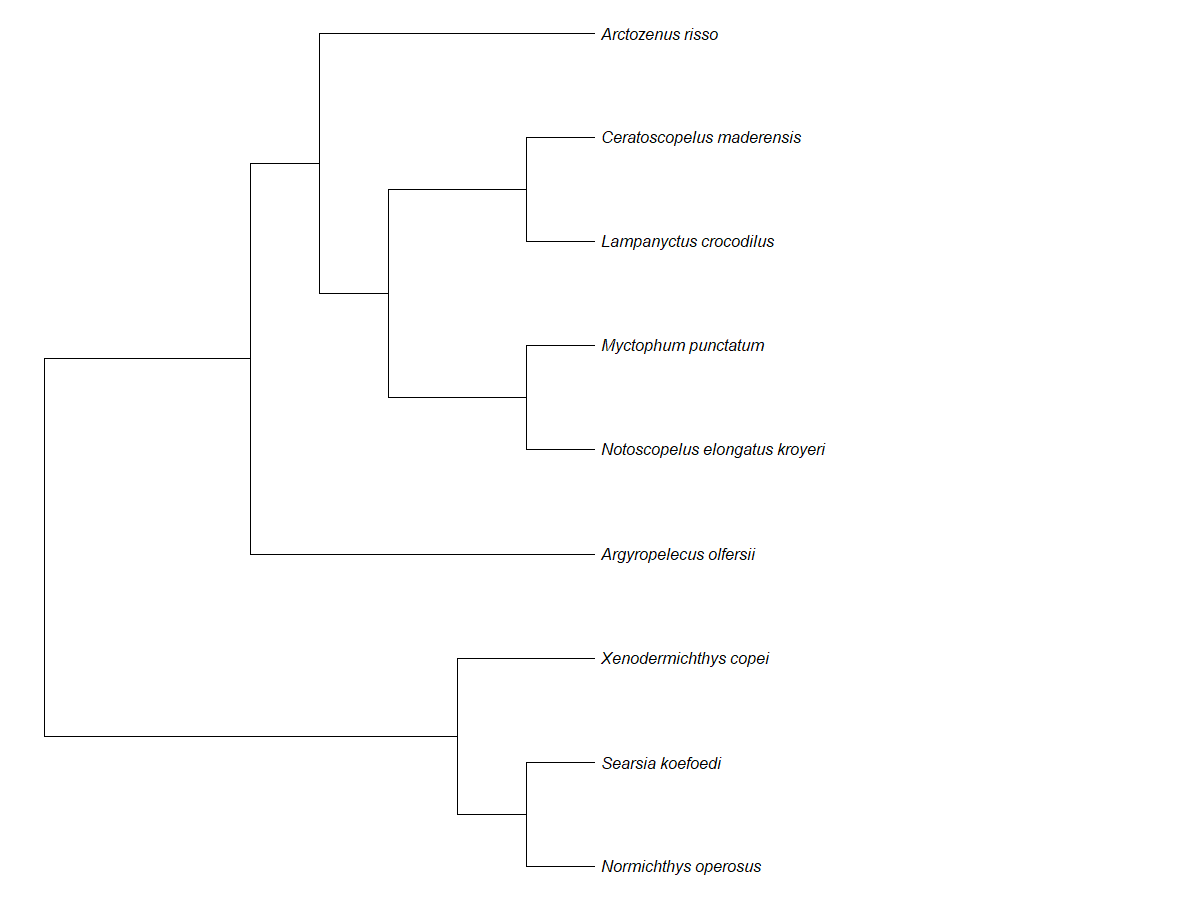
\includegraphics[width=0.8\textwidth]{phylogenic_tree.png}
	\end{center}
	\caption{Phylogenic tree of studied species, using R \emph{rotl} package~\citep{opentreeoflife2019}~.}
	\label{fig:phylotree}
\end{figure}


% \section{Morphological measurements}
%First figure: full body
\begin{figure} [!htbp]
	\begin{center}
		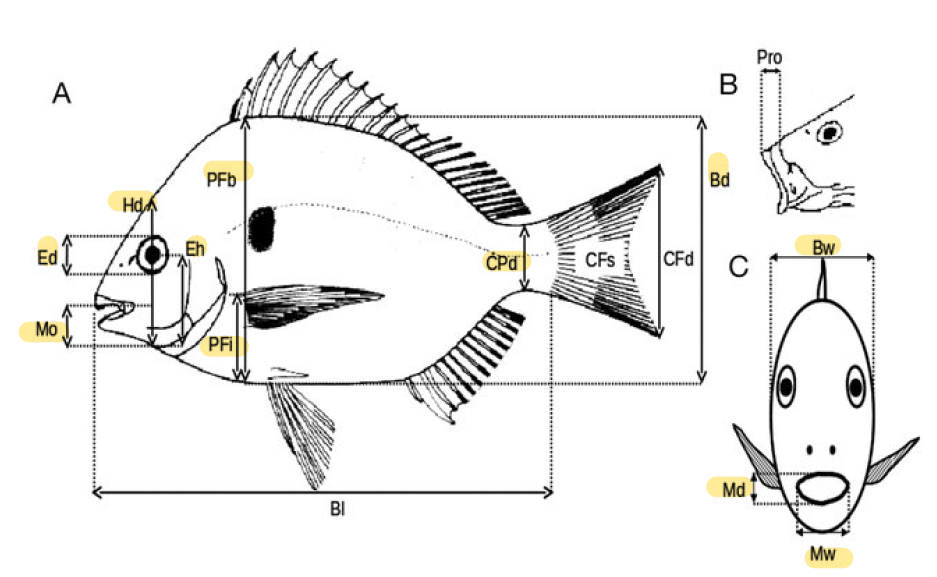
\includegraphics[width=0.8\textwidth]{Tp_Jerome_figure_1.png}
		\caption{Morphological measurements, from \citet{albouy2011}. \textsc{bd}, body depth; \textsc{bw}, body width;\textsc{cpd}, caudal peduncle minimal depth; \textsc{ed}, eye diameter; \textsc{eh}, distance between the bottom of the head and the eye center along the head depth axis; \textsc{hd}, head depth along the vertical axis of the eye; \textsc{md}, mouth depth; \textsc{mo}, distance between the tip of the upper jaw and bottom of the head; \textsc{mw}, mouth width; \textsc{pfb}, body depth at the level of the pectoral insertion; \textsc{pfi}, distance between the insertion of pectoral fin and the bottom of the body.}
	\label{fig:full_body}
	\end{center}
\end{figure}


%Second figure: zoom on the head
\begin{figure} [!htbp]
	\begin{center}
		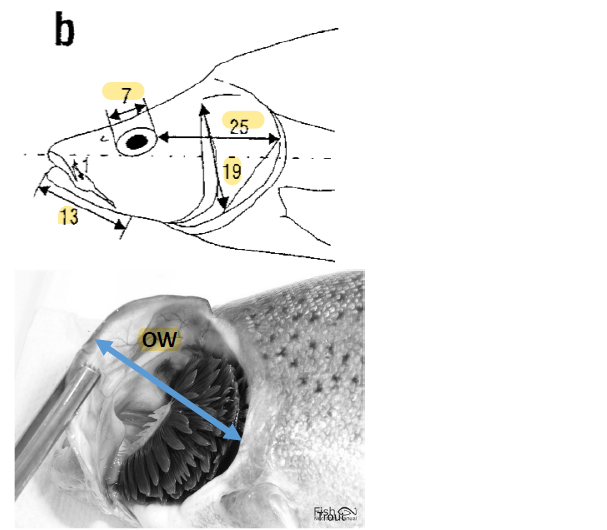
\includegraphics[width=0.8\textwidth]{Tp_Jerome_figure_2.png}
		\caption{Morphological measurements of the head, from \citet{diderich2006}, following \citet{sibbing2000}. 7 being \textsc{ed}, eye diameter; 13 \textsc{ljl}, distance between the tip and the insertion point of lower jaw; 19 \textsc{od}, depth of the operculum from point of insertion to bottom; 25 \textsc{pol}, shortest distance between the eye and the end of the head; \textsc{ow}, operculum maximum width.}
	\label{fig:head}
	\end{center}
	
\end{figure}


%Third figure: fin length
\begin{figure} [!htbp]
	\begin{center}
		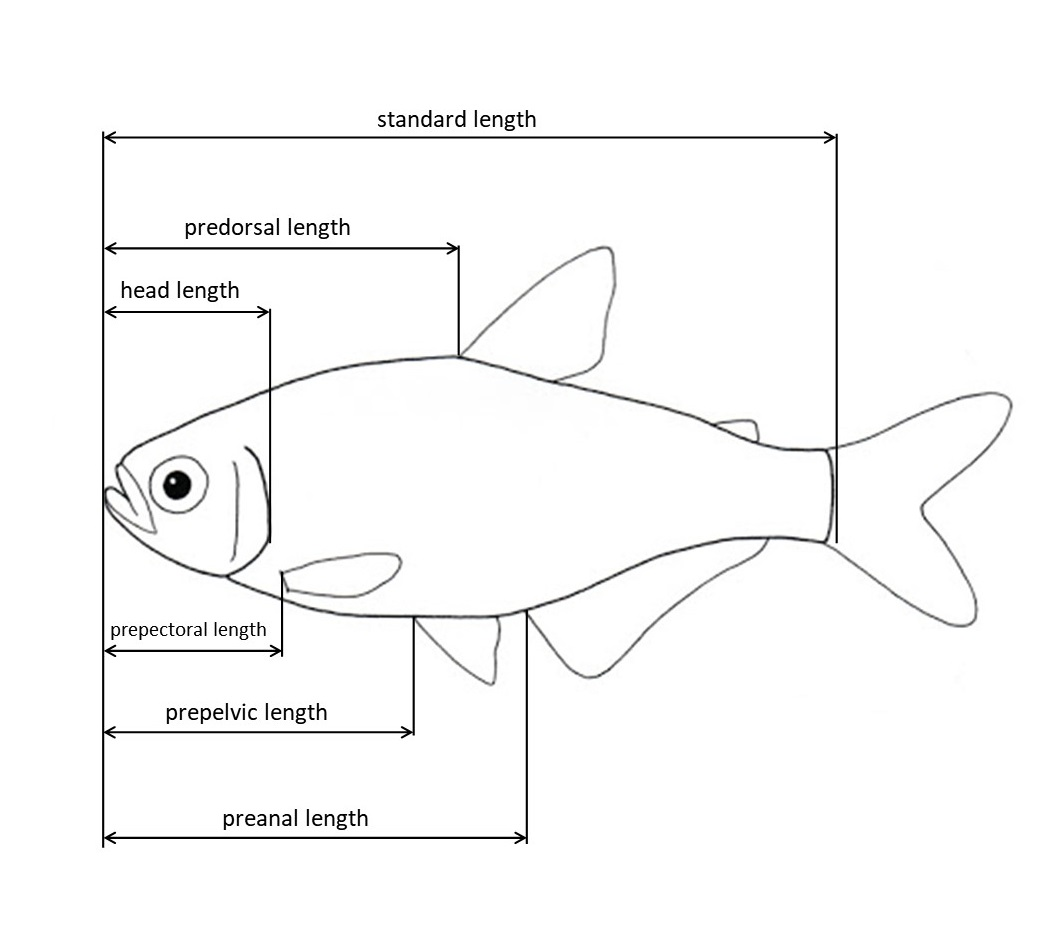
\includegraphics[width=0.8\textwidth]{Figure_3.jpg}
		\caption{Morphological measurements of the head, adpated from \citet{keat-chuanng2017,habib2019}. \textsc{hl}, head length, from the nose to the closest-to-caudal-fin point of the operculum; \textsc{pal}, distance bewteen the tip of the nose and the insertion of anal fin; \textsc{pdl}, distance bewteen the tip of the nose and the insertion of dorsal fin, \textsc{ppl}, distance bewteen the tip of the nose and the insertion of pectoral fin; \textsc{pvl}, distance bewteen the tip of the nose and the insertion of pelvic fin;  \textsc{sl}, standard length.}
		\label{fig:fin}
	\end{center}
	
\end{figure}


%Fourth and fifth figures: Git and OGA
\begin{figure} [!htbp]
	\begin{center}
	\begin{minipage}{0.45\textwidth}
		\centering
		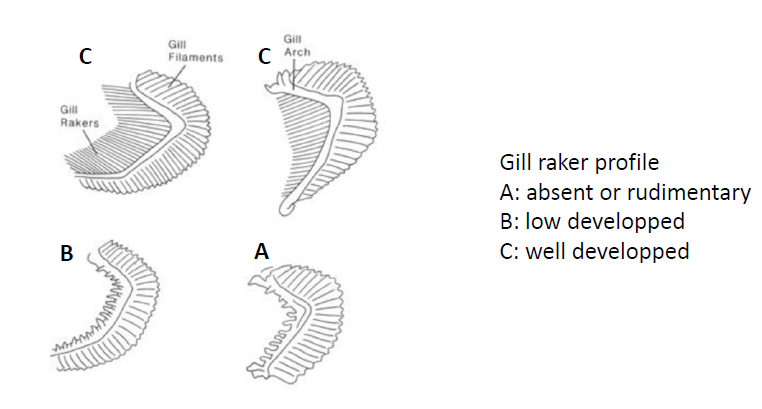
\includegraphics[width=1\textwidth]{Tp_Jerome_figure_Git.png}
		\caption[Petite légende]{Scores of gill rakers types \textsc{git}, based on their length.}
		\label{fig:git}
	\end{minipage}\hfill
	\begin{minipage}{0.45\textwidth}
		\centering
		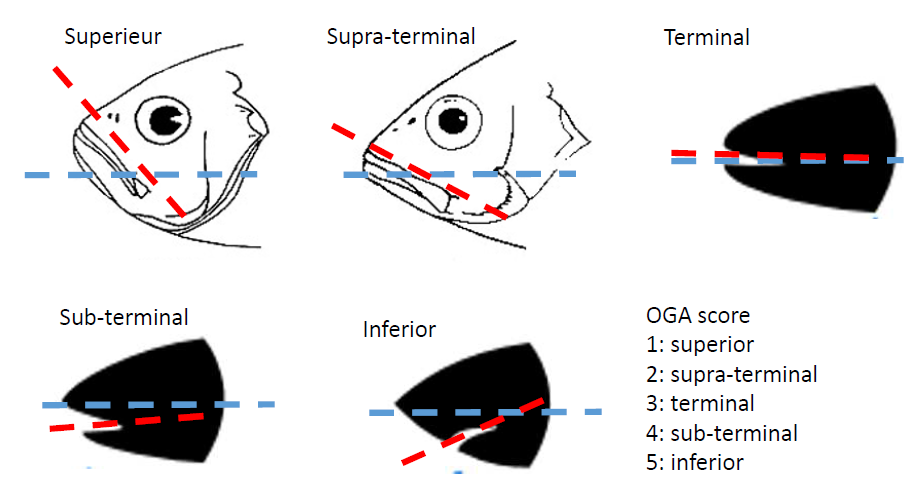
\includegraphics[width=1\textwidth]{Tp_Jerome_figure_Oga.png}
		\caption[Petite légende]{Scores of oral gape axis \textsc{oga}, based on the angle between mouth orientation (red) and a fictive mid-depth lateral lign (blue).}
		\label{fig:oga}
	\end{minipage}
	\end{center}
	
\end{figure}

% \section{Correlation plot}
% Correlation circle to help understand FAMD results
\begin{figure} [!htbp]
	\begin{center}
		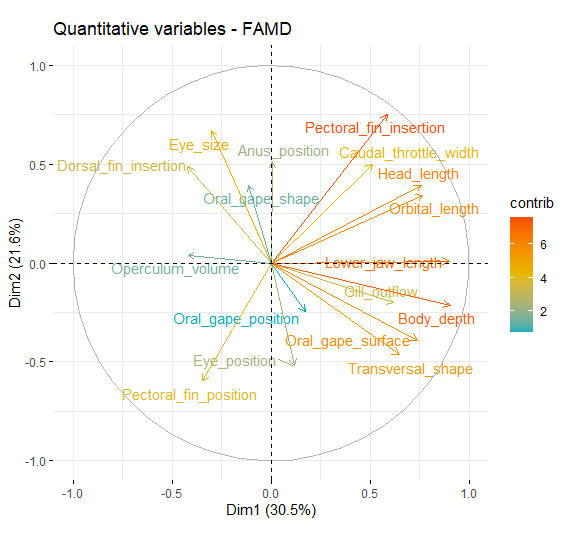
\includegraphics[width=0.8\textwidth]{Correlation_circle.png}
	\end{center}
	\caption{Correlation circle of axis 1 and 2. The 'contrib' variable refers to the representativity of the variable on the axis. The higher the value is, the more the corresponding variable contributes to the axis.}
	\label{fig:corr_circ_12}
\end{figure}

\begin{figure} [!htbp]
	\begin{center}
		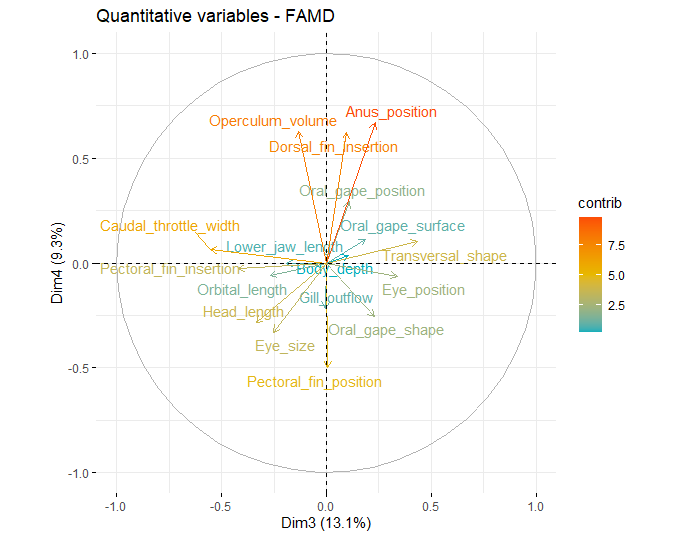
\includegraphics[width=0.8\textwidth]{coord_plot_34.png}
	\end{center}
	\caption{Correlation circle of axis 3 and 4. The 'contrib' variable refers to the representativity of the variable on the axis. The higher the value is, the more the corresponding variable contributes to the axis.}
	\label{fig:corr_circ_34}
\end{figure}






\bibliographystyle{molecularEcology}

% \begin{multicols}{2}
\bibliography{M2_Stage}
% \end{multicols}

% \section{Abstract}
% \section{Résumé}

\end{document}